% The generic preamble
\documentclass[10pt,letterpaper,fleqn,titlepage]{article}

% Define packages to use
\usepackage{natbib}
\usepackage[dvips]{graphicx,color}
\usepackage{amsmath,amssymb}
\usepackage{bm}
\usepackage{caption}
\usepackage{xr}
\usepackage{ifthen}
\usepackage[dvipdfm,colorlinks,linkcolor=blue,citecolor=blue,urlcolor=blue]{hyperref}
\usepackage{fancybox}
\usepackage{textcomp}
\usepackage{alltt}
%\usepackage{floatflt}
%\usepackage{svn}


% Redefine default page
\setlength{\textheight}{9in}  % 1" above and below
\setlength{\textwidth}{6.75in}   % 0.5" left and right
\setlength{\oddsidemargin}{-0.25in}

% Redefine default paragraph
\setlength{\parindent}{0pt}
\setlength{\parskip}{1ex plus 0.5ex minus 0.2ex}

% Define caption width and default fonts
\setlength{\captionmargin}{0.5in}
\renewcommand{\captionfont}{\sffamily}
\renewcommand{\captionlabelfont}{\bfseries\sffamily}

% Define commands for super- and subscript in text mode
\newcommand{\superscript}[1]{\ensuremath{^\textrm{#1}}}
\newcommand{\subscript}[1]{\ensuremath{_\textrm{#1}}}

% Derived commands
\newcommand{\invcm}{\textrm{cm\superscript{-1}}}
\newcommand{\micron}{\ensuremath{\mu\textrm{m}}}

\newcommand{\df}{\ensuremath{\delta f}}
\newcommand{\Df}{\ensuremath{\Delta f}}
\newcommand{\dx}{\ensuremath{\delta x}}
\newcommand{\Dx}{\ensuremath{X_{max}}}
\newcommand{\Xeff}{\ensuremath{X_{eff}}}

\newcommand{\water}{\textrm{H\subscript{2}O}}
\newcommand{\carbondioxide}{\textrm{CO\subscript{2}}}
\newcommand{\ozone}{\textrm{O\subscript{3}}}

\newcommand{\taup}[1]{\ensuremath{\tau_{#1}}}
\newcommand{\efftaup}[1]{\ensuremath{\tau_{#1}^{*}}}

\newcommand{\textbfm}[1]{\boldmath\ensuremath{#1}\unboldmath}

\newcommand{\rb}[1]{\raisebox{1.5ex}[0pt]{#1}}

\newcommand{\f}[1]{\texttt{#1}}

% Define how equations are numbered
\numberwithin{equation}{section}
\numberwithin{figure}{section}
\numberwithin{table}{section}

% Define a command for title page author email footnote
\newcommand{\email}[1]
{%
  \renewcommand{\thefootnote}{\alph{footnote}}%
  \footnote{#1}
  \renewcommand{\thefootnote}{\arabic{footnote}}
}

% Define a command to print the Office Note subheading
\newcommand{\notesubheading}[1]
{%
  \ifthenelse{\equal{#1}{}}{}
  { {\Large\bfseries Office Note #1\par}%
    {\scriptsize \sc This is an unreviewed manuscript, primarily intended for informal}\\ 
    {\scriptsize \sc exchange of information among JCSDA researchers\par}%
  }
}

% Redefine the maketitle macro
\makeatletter
\def\docseries#1{\def\@docseries{#1}}
\def\docnumber#1{\def\@docnumber{#1}}
\renewcommand{\maketitle}
{%
  \thispagestyle{empty}
  \vspace*{1in}
  \begin{center}%
     \sffamily
     {\huge\bfseries Joint Center for Satellite Data Assimilation\par}%
     \notesubheading{\@docnumber}
  \end{center}
  \begin{flushleft}%
     \sffamily
     \vspace*{0.5in}
     {\Large\bfseries\ifthenelse{\equal{\@docseries}{}}{}{\@docseries: }\@title\par}%
     \medskip
     {\large\@author\par}%
     \medskip
     {\large\@date\par}%
     \bigskip\hrule\vspace*{2pc}%
  \end{flushleft}%
  \newpage
  \setcounter{footnote}{0}
}
\makeatother
\docseries{}
\docnumber{}


% Define a command for a DRAFT watermark
\usepackage{eso-pic}
\newcommand{\draftwatermark}
{
  \AddToShipoutPicture{%
    \definecolor{lightgray}{gray}{.85}
    \setlength{\unitlength}{1in}
    \put(2.5,3.5){%
      \rotatebox{45}{%
        \resizebox{4in}{1in}{%
          \textsf{\textcolor{lightgray}{DRAFT}}
        }
      }
    }
  }
}





% Title info
\title{Coding Review and Acceptance Guidelines}
\author{Paul van Delst\email{paul.vandelst@noaa.gov}\\JCSDA/EMC/SAIC}
\date{January, 2008}
\docseries{CRTM}


%-------------------------------------------------------------------------------
%                            Ze document begins...
%-------------------------------------------------------------------------------
\begin{document}
\maketitle

\draftwatermark
  

\section{Motivation}
%===================
Manage the workload and potential for interruption due to ongoing development of the CRTM.  


\section{Code Review Process}
%============================
\label{sec:code_review_process}
The following details the proposed procedure for development and acceptance of source code for use in a CRTM release.
\begin{itemize}
  \item Prior to any coding
  \begin{itemize}
    \item Developer shall propose changes in advance. For significant changes, a design review should be held to ensure the proposed changes will integrate into the CRTM; or, alternatively, suggest alterations to the internal structure of the CRTM to accomodate the developer's code.
    \item Developer shall adhere to CRTM Coding Guidelines\cite{CRTM_Coding_Guidelines}.
    \item Developer shall update their CRTM working copy to the repository head revision and ensure that tests pass. For significant changes, a repository branch will be created for the developer.
  \end{itemize}
  \item Prior to any CRTM trunk commit
  \begin{itemize}
    \item Developer shall make updated code available to other developers for optional review.
    \item For a significant change (i.e. not just a simple bug fix), the developer shall make working code available to other developers with enough lead time to permit review before the desired commit date.
    \item Developer shall add new tests to test suite for new features.
    \item Interested developers may review the code and suggest modifications.
    \item Developers who are responsible for a section of code may require changes.
    \item Proposed changes are discussed. Meeting schedule for this needs to be determined (e.g. regular, or as required?). Changes that are ready to commit are ordered.
  \end{itemize}
  \item Person responsible for a particular section of code has veto power of commit.
  \item After all commits are completed, JCSDA CRTM core developers shall run an extensive suite of tests.
  \item Any test failures exposed by the extensive suite shall be fixed by the original developer(s).
\end{itemize}


\section{Code Selection Criteria}
%================================
\label{sec:code_selection_criteria}
\textcolor{red}{This section needs some quantitative guidance from operational users.Additional, or more useful criteria?}

Currently, there are three categories of code acceptance criteria.

\subsection{Review}
%------------------
\begin{itemize}
  \item Clarity. Is the code understandable?
  \item Maintainability. Is the code designed for easy maintenance?
\end{itemize}
These criteria are somewhat subjective but, as stated, they can be satisfied via iterations of the code review process discussed in section \ref{sec:code_review_process}.

\subsection{Specification}
%-------------------------
\begin{itemize}
  \item Speed. Is it fast enough?
  \item Accuracy. Is it accurate enough?
  \item Memory usage. Does it use too much memory?
\end{itemize}
To be useful, the specification criteria obviously need to be quantified but the relative importance of each is dependent on the application. A two-tiered approach is suggested.

Firstly, what are the limits that would cause current operational codes to fail? That is, if the code is too slow then much less satellite data will make it into the data assimilation system eventually degrading the forecast; or if the code uses too much memory, page faulting causes it to halt.

Secondly, what are the margins that developers can use to guide their development? Determining these numbers is a bit more difficult as it depends on the application and the user's hardware.

\textcolor{red}{A chart of typical/suggested values for the different JCSDA partners?}


\subsection{Testing}
%-------------------
\subsubsection{Baseline model tests}
%...................................
Code should be provided that runs the CRTM module under development and compares it with  supplied results that are known to be correct.

\textcolor{red}{Baseline test for all components, i.e. forward, tangent-linear, adjoint, K-matrix (if appropriate)? Or just the forward model since the following should test for the others?}


\subsubsection{Forward/Tangent-linear test}
%..........................................
Let $F(x)$ represent the forward model for input $x$, and $TL(\delta x)$ represent the tangent-linear model for perturbation input $\delta x$. The relationship
\begin{equation}
  \frac{F(x+\alpha\cdot\delta x) - F(x)}{\alpha\cdot TL(\delta x)} = 1+O(\alpha)
\end{equation}
should be true, where $\alpha = 0.1,0.01,0.001,$\ldots

\subsubsection{Tangent-linear/Adjoint Test}
%..........................................
Let $\mathbf{TL(\delta x)}$ represent the tangent-linear model result for perturbation input vector  $\mathbf{\delta x}$, and $\mathbf{AD\left(TL(\delta x)\right)}$ represent the adjoint model result where the tangent-linear model output is used as adjoint model input. The following relationship,
\begin{equation}
  \mathbf{TL(\delta x)^{t}\cdot TL(\delta x) = \delta x^{t}\cdot AD\left(TL(\delta x)\right)}
\end{equation}
must be true to within numerical precision.

\subsubsection{Adjoint/K-matrix Test}
%....................................
For specified adjoint input, $\delta y^{*}$, let $AD(\delta y^{*})$ represent the adjoint model result, and $K_{l}(\delta y^{*})$ the K-matrix result for sensor channel $l$. The following relationship
\begin{equation}
  AD(\delta y^{*}) = \sum_{l=1}^{L} K_{l}(\delta y^{*})
\end{equation}
must be true to within numerical precision. 


\section{Repository Organisation}
%================================
The top-level CRTM repository structure is shown in figure \ref{fig:CRTM_Repository_Structure}. This type of structure is standard for repositories in general\cite{SubversionManual,Mason2005}. The naming of branches and tags as shown in figure \ref{fig:CRTM_Repository_Structure} is also a \textit{de facto} standard (see \cite{Mason2005} for additional examples) that emphasises convention over configuration. That is, any developer should be able to inspect the repository and determine branch and tag information from their names.
\begin{figure}[htp]
  \hfill
  \begin{minipage}[t]{.475\textwidth}
    \begin{center}
      \includegraphics[scale=0.8]{graphics/CRTM_Repository_Structure.eps}
    \end{center}
  \end{minipage}
  \hfill
  \begin{minipage}[b]{.475\textwidth}
    \begin{itemize}
      \item Three main directories
        \begin{itemize}
          \item trunk
          \item branches
          \item tags
        \end{itemize}

      \item trunk
        \begin{itemize}
          \item The main line of development
          \item Subdirectories here are based on logical association of what different CRTM components do (e.g. AtmOptics, SfcOptics, etc.)
        \end{itemize}

      \item branches
        \begin{itemize}
          \item This is where branches go.
          \item Experimental development branches with name \textsf{EXP-}\emph{desc}
          \item Other branches related to code releases with name \textsf{RB}-\emph{rel}
        \end{itemize}

      \item tags
        \begin{itemize}
          \item This is where snapshots and releases go.
          \item Snapshots. \textsf{REL-rev}\emph{num}.\emph{YYYY-MM-DD}
          \item Releases. \textsf{REL-}\emph{rel}
          \item No development (otherwise it would be a branch.)
        \end{itemize}
    \end{itemize}
  \end{minipage}
  \caption{Example and description of top-level directory structure of the CRTM Subversion repository.}
  \label{fig:CRTM_Repository_Structure}
  \hfill
\end{figure}


\section{Repository Access}
%==========================
\subsection{Policy}
\begin{itemize}
  \item To start with, developers will have \textbf{read-only} access. It is acknowledged that this restriction works against agile development\footnote{That's agile with a lower case ``a''. It should not be confused with the Agile Development framework for software engineering. See \href{http://en.wikipedia.org/wiki/Agile_software_development}{http://en.wikipedia.org/wiki/Agile\_software\_development}}, but until there are sufficient test cases it's a necessary evil.
  \item Until write-access is granted, code to be considered for commit is provided as a tarball uploaded to CRTM ftp site.
  \item CWG co-chairs responsible for repository branch creation. Developers request a branch for write-access.
\end{itemize}

\subsection{Details}
\begin{itemize}
  \item Offsite Subversion repository.
  \item SCM software \textcolor{red}{\textbf{this is important!}}
  \item Website/wiki for online CRTM documentation.
  \item ftp site for release download, or code upload.
  \item User forum.
\end{itemize}
We need this capability to be \emph{much} more flexible than it is now. IT security restrictions have hampered CRTM development. This is not an indictment of the current security protocols and procedures - they are there for a reason - but the current status quo is slowing development.


\section{Code Release Policy}
%============================
\textcolor{red}{This section needs better organisation}
\begin{itemize}
  \item All releases will be made from the top of the main trunk of the repository. All developers will be notified in advance of any type of release.  

  \item Prior to every release, a release branch will be created for pre-release testing. During this pre-release stage, the the main trunk of the repository will still be available for development. Bug-fixes in either the current release branch or trunk shall be merged.

  \item In order to allow time for developers to test modifications on their machines and contribute bug fixes in time for pre-release testing, all releases must be announced at least two months in advance.

  \item All components of the CRTM will be released together.  

  \item A ``major release'' contains important new scientific and/or software engineering advancements that significantly alter the behavior and/or performance of the CRTM. Numbering for major releases increments the first element of the version number.  Examples:  ``CRTM 2.0.0'', ``CRTM 3.0.0''. Major releases will be synchronized across all development subgroups and scheduled well in advance. There will be no more than one major release per year.  

  \item A ``minor release'' contains minor feature additions and enhancements. Model behavior is not fundamentally altered.  Numbering for minor releases increments the second element of the version number.  Examples:  ``CRTM 2.1.0'', ``CRTM 3.2.0''. Minor releases will be scheduled well in advance and will be coordinated across all developers.  However it is not required that every subgroup schedule minor releases at the same time.  This allows for quicker turnaround of minor feature enhancements by individual development subgroups.  

  \item A ``patch release'' contains bug fixes.  No new features are added. Coordination and scheduling are identical to minor releases, except that less advance notice is required. This allows for quick turnaround of bug fixes by individual development subgroups. Numbering for patch releases increments the third element of the version number.  Examples:  ``CRTM 2.1.1'', ``CRTM 2.1.2''

  \item Release numbering and designation of the type of releases is primarily the responsibility of the CRTM Working Group.
  
  \item For all releases, the full CRTM test suite must be run on all supported platforms.  

  \item For major releases, the CWG will run the full CRTM test suite on all supported platforms.

  \item For minor and patch releases, the development subgroup that has requested the release is responsible for running the full CRTM test suite on all supported platforms.  

  \item The CWG is responsible for content of the CRTM test suite.  

  \item No policy is perfect.  Variations from this policy will be allowed with prior consent from all affected subgroups.  
\end{itemize}

\section{Policy Consequences}
%============================
It must be possible for a development subgroup to make a minor release or a patch release without seriously impacting development schedules in other subgroups.  Therefore, the main trunk of the repository must always contain source code that is suitable for release, or nearly so.  

Development that is not yet ready for release must be done in a repository branch or in a checked-out working copy.  The use of repository branches for any non-trivial development is strongly encouraged.  



%
%WRF Merge-Test-Commit Procedure
%         1)  Merge ("update" in revision control lingo) sandbox/branch to the head 
%             of the main trunk of the repository.  (The first developer must have 
%             already done this.)  (See here for more information about the CVS 
%             "update" command.)
%         2)  Run regtest.csh on the merged code.  (The first developer must have 
%             already done this.)  (See here for more information about WRF testing.)  
%               a)  For a "software engineering" change (that should not affect model
%                   results), run regtest.csh to generate a "baseline" data set and
%                   then run regtest.csh again to compare modified code with the
%                   baseline:
%                     i)  Generate a "baseline" data set by running regtest.csh from
%                         the head of the main trunk.  To generate a baseline, edit
%                         regtest.csh and change the line that sets GENERATE_BASELINE
%                         to point to a directory that does not already exist.  For
%                         example, the following edit will write a baseline data set
%                         to directory /ptmp/hender/WRF_BASELINE_20051122_1001 :
%> set GENERATE_BASELINE = FALSE
%< set GENERATE_BASELINE = /ptmp/hender/WRF_BASELINE_20051122_1001
%                     ii) Compare against the "baseline" data set by running regtest.csh
%                         from the newly modified code.  edit regtest.csh and change
%                         the line that sets COMPARE_BASELINE to point to a directory
%                         that contains previously generated baseline data.  For
%                         example, the following edit will compare against a baseline
%                         data set in directory /ptmp/hender/WRF_BASELINE_20051122_1001 :
%< set COMPARE_BASELINE = FALSE
%> set COMPARE_BASELINE = /ptmp/hender/WRF_BASELINE_20051122_1001
%                         Note that both GENERATE_BASELINE and COMPARE_BASELINE should
%                         not both be set to a directory at the same time.
%               b)  For a "science" change (that does affect model results), simply run
%                   regtest.csh once and ensure that it does not fail.  (We will
%                   eventually have real tests for science changes.)
%         3)  Commit ("check in" changes to the main trunk of the repository.  (See here 
%             for more information about the CVS "commit" command.)  
%         4)  Tag the main trunk of the repository.  In CVS, tags make it much easier to 
%             merge changes between branches and the main trunk.  (Note that this will not 
%             be necessary once we move to Subversion.)  The tag naming convention is:  
%               trunk_yyyymmdd_ii 
%             Where "yyyymmdd" is time-date and "ii" is developer initials.  From a working 
%             copy (sandbox) checked out from the main trunk, the following cvs command 
%             illustrates syntax for a commit made by developer "TH" on 12/02/2005:  
%>> cvs tag trunk_20051202_th
%         5)  Remaining developers each follow steps 1-4 to merge, test, commit, and tag 
%             their changes.  
%         6)  Once all commits have been made, the "floating chairperson" will run the
%             full "all_reg" set of tests on the head of the main trunk.  Any failures
%             will be referred back to the developers for fixing.
%             Note that requiring individual users to run all_reg is also an option.
%             The decision to require only regtest is a tradeoff of test coverage vs.
%             test time.  We may choose to adjust this tradeoff if all_reg starts
%             finding too many errors.
%
%   - As indicated in the above procedure, we will continue to require that 
%     main trunk changes pass regression tests prior to commit.  See 
%     http://box.mmm.ucar.edu/wrf/WG2/allreg/tests.html for more details about 
%     WRF testing.  Exceptions to this rule include changes that have no 
%     possibility of adversely impacting other developers (such as changes 
%     to comments, etc.).  
%   - Developers are largely free to do whatever they want on their own 
%     repository branches.  I have posted best-practice recipes for creating, 
%     updating, and merging CVS repository branches on the WRF web pages.  A few 
%     key issues:  
%     - Update branches from the main trunk weekly.  Otherwise, updating can 
%       become very difficult.  
%     - Record the latest main-trunk update point in each branch.  CVS does not 
%       maintain this information, which is critical for merging.  This can be 
%       done in the CVS check-in messages.  
%     - Do not copy CVS directories between working copies.  This is a good way 
%       to scatter changes across multiple branches when committing.  Clean-up 
%       can be very labor-intensive.  
%   - The main trunk of the WRF repository is theoretically considered to be 
%     releasable at any moment (though in practice, all releases will be 
%     coordinated).  Work that is not suitable for public distribution (such as 
%     unpublished research results) should not be committed to the main trunk.  
%   - NCAR will run automated regression tests weekly on the HEAD of the main 
%     trunk of the repository to ensure that it remains stable.  This will only 
%     be done when the HEAD of the main trunk had changed since the last time 
%     the tests were run.  
%
%
%Heavier-Weight Process Options
%
%  If we can all behave nicely together, the above lightweight process should 
%  suffice.  However, if needed, we can consider adding one or more of the 
%  following to the process:  
%   - Post a long-term development schedule on the web to improve 
%     communication among developers.  For example, see:
%       http://www.cgd.ucar.edu/~cam/cam_checkins/
%   - Run automated regression tests nightly on the HEAD of the main trunk of 
%     the repository to ensure that it remains stable.  This would only be done 
%     when the main trunk had changed since the last time the tests were run.  
%   - Institute formal code review, possibly including a formal change-review
%     board.  This ought not to be necessary for such a small development
%     effort.  Such a process might mirror the current WRFVAR process:  
%       WRFVAR process:  
%       a) Developer proposes changes with draft of methodology and impact in 
%          prototype tests (if any).  
%       b) If approved for potential inclusion, a reviewer is assigned and 
%          development schedule decided.  
%       c) Contributed code is merged up to the head of the repository main 
%          trunk and tested using the WRF test suite.  If the new code changes 
%          scientific results, additional tests which show the new capability 
%          in action are also required.  
%       d) Developer and reviewer present results to the relevant working 
%          group or change review board.  
%       e) When approved, changes are added to repository (including a change 
%          file describing code changes and impacts).
%
%
%
%
%

\section*{Acknowledgement}
%=========================
Many of the guidelines and policies in this document were adapted from those for the original WRF Source Code Control Procedures available at:

\href{http://box.mmm.ucar.edu/wrf/WG2/allreg/WRFSourceCodeControlPolicies.html}{http://box.mmm.ucar.edu/wrf/WG2/allreg/WRFSourceCodeControlPolicies.html}


% The references section
%=======================
\bibliographystyle{plain}
\bibliography{bibliography}

% The appendices section
%=======================
\begin{appendix}
\end{appendix}

\end{document}

